\section{Methodology}

This section describes some of the theory and methods involved in this work. The governing equations of the numerical model presented here are discussed in section \ref{subsec:LTE}. Following this, a description of the equations discretisation and the numerical scheme required to solve them are outlined in section \ref{subsec:model}.

\subsection{Laplace Tidal Equations \label{subsec:LTE}}

The equations of motion and mass conservation that describe ocean flow in the shallow water limit are called the Laplace Tidal Equations (LTE) (also known as the shallow water equations) \citep{lamb1932hydrodynamics}. The main assumption in their derivation is that radial (vertical) ocean flow is negligible when compared to lateral flow. This is indeed a good approximation for global oceans, where lateral flow spans a much greater distance than the depth of the ocean. The conservation of mass (eq. \ref{eq:mass}) and momentum (eq. \ref{eq:mom}) that make up the LTE, including both Rayleigh and bottom friction, are given as \citep{sears1995tidal,tyler2008strong,matsuyama2014tidal}:

%Adds vertical space between equations
%\setlength{\jot}{8pt}
%environment centres all equations

\vspace{-0.5cm}
\begin{gather}
\partial_t \eta + \nabla \cdot \left(h \bm{u}\right) = 0\, , \label{eq:mass}\\
\begin{aligned} 
\partial_t \bm{u} + 2 \bm{\Omega} \times \bm{u} + \alpha\bm{u} + \frac{c_D}{h} \left|\bm{u}\right| \bm{u}  + g \nabla \eta \\ = (1 + k_2 - h_2) \nabla U_2 \, . \label{eq:mom}\\
\end{aligned} 
\end{gather}

Equation \ref{eq:mass} consists of two terms. The first is the time rate of change of vertical sea surface displacement about some equilibrium level. $\eta$ denotes this displacement. The second term represents the divergence of the surface velocity vector, $\bm{u} \equiv (u, v)$, where $u$ and $v$ are the eastward and northward velocity components respectively. In our calculations, we assume the ocean's undisturbed depth, $h$, to be constant. 

The term on the right hand side of Equation \ref{eq:mom} is an applied force per unit mass. $\nabla U_2$ is the gradient of the degree-2 tidal potential (discussed in section ...). It is multiplied by Love's reduction factor involving the degree-2 tidal Love numbers, $k_2$ and $h_2$. Love's first number, $k_2$, is a proportionality constant accounting for the additional tidal potential due to the elastic redistribution of mass on the satellite. $h_2$, the second Love number, accounts for the tidal potential arising from solid body surface displacement of the satellite \citep{love1911some}.

The time derivative of velocity is given by the first term on the left hand side of the momentum equation. It is balanced by four other acceleration per unit mass terms on the left hand side. The first of these terms is the coriolis acceleration per unit mass, where $\Omega$ is the satellite's rotational angular velocity. Rayleigh and bottom friction are described in the next two terms, where $\alpha$ and $c_D$ are the Rayliegh (linear)and bottom (quadratic) friction coefficients respectively \citep{sears1995tidal,chen2013tidal}. The last term on the right hand side of Equation \ref{eq:mom} is the gravitational restoring acceleration per unit mass. It acts to balance changes in sea surface displacement, given by the gradient of equilibrium displacement, $\nabla \eta$ .

\subsection{Numerical Model \label{subsec:model}}

The numerical model outlined below is based on the models extensively discussed in \citet{zahel1973diurnalk,zahel1978influence} and \citet{sears1994tidal,sears1995tidal}. In this section we first provide a description of the numerical grid setup, before giving an overview of the finite difference scheme itself.

\subsubsection{Discretized Grid}

\begin{figure*}[t]
\centering
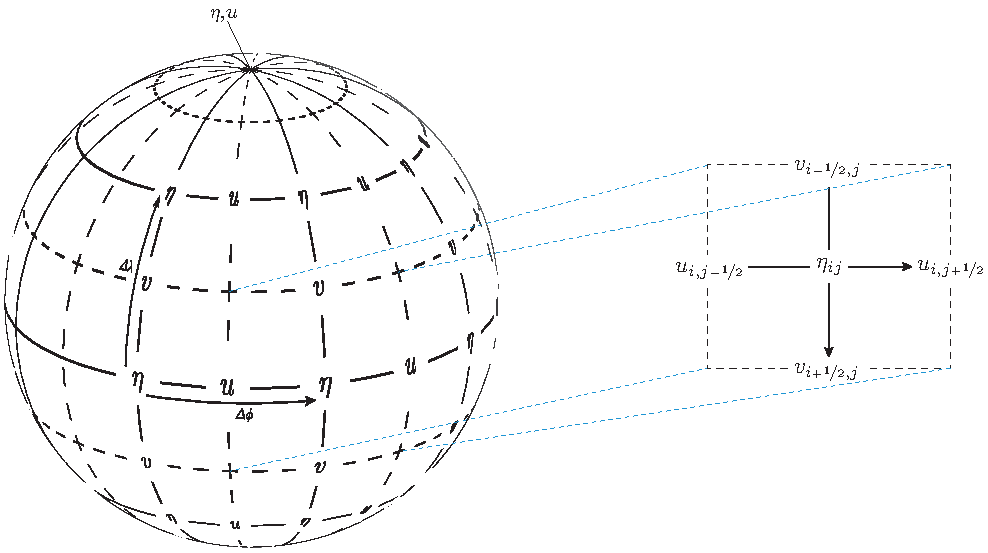
\includegraphics[width = 0.8\linewidth]{Figures/GridDiagram}
\caption{The staggered grid structure used in ODIS. A single cell is show on the right of the figure, where surface displacement, $\eta$, represents a cell centered quantity. $u$ velocity nodes are staggered eastward of $\eta$, whereas $v$ velocity nodes are staggered southwards. Both $u$ and $v$ are defined at the cell walls. Lines of meridian merge to singularities at the pole, which contain both $u$ and $\eta$ quantities.}
\end{figure*}

We made grid. 

\subsubsection{Finite Difference Expansions}

As in \citep{sears1995tidal}, we expand equations \ref{eq:mass} and \ref{eq:mom} in a semi-implicit finite difference scheme in spherical coordinates. By expanding $\bm{u}$ into its components, the momentum equation becomes,

\vspace{-0.6cm}
\begin{multline}
u_{ij}^{t+1} \approx  \left[ \,2 \Omega \bar{v}_{ij} \sin{\lambda_i} \vphantom{\frac{c_D}{h}\sqrt{\left(u_{ij}^{t}\right)^2}} - \alpha u_{ij}^{t} \right. \\ 
- \frac{c_D}{h}\sqrt{\left(u_{ij}^{t}\right)^2 + \left(\bar{v}_{ij}^{t}\right)^2}\cdot\left(u_{ij}^{t}\right)^2 - \frac{g}{R \cos{\lambda_i}} \frac{\partial \eta_{ij}^{t}}{\partial \phi_j} \\  
+ \left.\left(1 + k_2 - h_2\right) \frac{1}{R \cos{\lambda_i}} \frac{\partial U_{2,ij}^{t}}{\partial \phi_j} \right]  \Delta t + u_{ij}^{t} \, , \label{eq:momu_fd}
\end{multline}
\vspace{-0.6cm}
\begin{multline}
v_{ij}^{t+1} \approx  \left[ \,-2 \Omega \bar{u}_{ij} \sin{\lambda_i} \vphantom{\frac{c_D}{h}\sqrt{\left(u_{ij}^{t}\right)^2}} - \alpha v_{ij}^{t} \right. \\ 
- \frac{c_D}{h}\sqrt{\left(\bar{u}_{ij}^{t}\right)^2 + \left(v_{ij}^{t}\right)^2}\cdot\left(v_{ij}^{t}\right)^2 - \frac{g}{R} \frac{\partial \eta_{ij}^{t}}{\partial \lambda_i} \\  
+ \left.\left(1 + k_2 - h_2\right) \frac{1}{R} \frac{\partial U_{2,ij}^{t}}{\partial \lambda_i} \right]  \Delta t + v_{ij}^{t} \, , \label{eq:momv_fd}
\end{multline}

and the mass conservation equation becomes, 
\begin{equation}
\eta_{ij}^{t+1} \approx 
-\frac{h}{R \cos{\lambda_i}}\left(
\frac{\partial \left(v_{ij}^{t+1} \cos{\lambda_i}\right)}{\partial	\lambda_i}  
+\frac{\partial u_{ij}^{t+1}}{\partial	\phi_j}\right)
\Delta t
+ \eta_{ij}^{t}\, . \label{eq:mass_fd}
\end{equation}

Latitude and longitude are denoted by $\lambda$ and $\phi$ respectively. $i$ and $j$ represent the $i\text{th}$ and $j\text{th}$ latitude and longitude positions within the grid. The time index is given by $t$, and $\Delta t$ represents the time-step. Overbars correspond to averages, a necessity given the staggered nature of the grid.

All derivatives of the degree-2 tidal potential have analytical solutions (section ...), and thus do not require further finite difference expansions. Derivatives of all other quantities, however, do require further expansion. The expansions take the general form of either,

\begin{align}
\frac{\partial w_{ij}}{\partial \lambda} &\approx \frac{w_{i+\nicefrac{1}{2},j} - w_{i-\nicefrac{1}{2},j}}{\Delta \lambda} \, , \label{eq:gen1}
\shortintertext{or, }
\frac{\partial w_{ij}}{\partial \phi} &\approx \frac{w_{i,j+\nicefrac{1}{2}} - w_{i,j-\nicefrac{1}{2}}}{\Delta \phi} \, , \label{eq:gen2}
\end{align}

where $w$ represents $u$, $v$ or $\eta$. $\Delta \lambda$ and $\Delta \phi$ are the latitude and longitude grid spacing, respectively. 

Examining equations \ref{eq:gen1} and \ref{eq:gen2} reveals that each derivative is evaluated halfway between the grid points where $w$ is stored. Consequently, any derivative of $w$ is calculated at the grid position held by a different function. For example, $\partial_\phi u_{ij}$ is always evaluated at the position held by $\eta_{ij}$ as $u_{i,j-\nicefrac{1}{2}}$ and $u_{i,j+\nicefrac{1}{2}}$ lie to the left and right of $\eta_{ij}$,  respectively. This is best visualized in figure ...

\subsubsection{Numerical Scheme}

ODIS begins its calculations by determining the mass of each volume element in the initial ocean, whether it be undisturbed or from some other initial condition. With the mass calculated in each cell, it is then possible to update the Rayleigh or bottom friction dissipated energy.

The next step in the numerical integration is to calculate $\nabla U_2$ across all $u$ and $v$ grid points. This gives the initial force per unit mass experienced by an element in the model domain.

Once the tidal forcing is known, ODIS directly calculates $u$ and $v$ over the grid by solving equations \ref{eq:momu_fd} and \ref{eq:momv_fd}. This step is purely explicit as $u$ and $v$ depend only on information from the previous time step, $t$. Following this, $\eta$ is then updated using the new velocity values. In contrast to the velocity calculations, this step is semi-implicit as it relies on both values from the current and previous time steps, as shown in Equation \ref{eq:mass_fd}.

After the solutions for $u$, $v$, and $\eta$ are found at the new time step, $t+1$, the energy calculations begin. For Rayleigh friction, we calculate and store dissipated energy as,
\begin{equation}
\dot{E}_{\alpha}^{t+1} = \frac{1}{4 \pi R^2 }\sum_{i=1}^{n} \sum_{j=1}^{m} \alpha m_{ij} \left[\left(u_{ij}^{t+1}\right)^2 + \left(v_{ij}^{t+1}\right)^2\right] \, , \label{eq:E_alpha}
\end{equation}

for $n$ and $m$ grid points in latitude and longitude, respectively. 

The summed terms in Equation \ref{eq:alpha_E} give the total dissipated energy in the system across the current time step, while the factor in front averages this quantity over the satellites surface area giving a quantity in watts per square metre. For bottom friction the equivalent expression is,
\begin{equation}
\dot{E}_{c_D}^{t+1} = \frac{1}{4 \pi h R^2 }\sum_{i=1}^{n} \sum_{j=1}^{m} c_D m_{ij} \left[\left(u_{ij}^{t+1}\right)^2 + \left(v_{ij}^{t+1}\right)^2\right]^{\nicefrac{3}{2}} \label{eq:E_cd}
\end{equation}
Details of these derivations are discussed in the appendix.

All previous steps are completed every time step. Finally, at the end of each orbit, $\dot{E}_\alpha$ or $\dot{E}_{c_D}$ is summed and averaged over the orbital period. This gives the orbitally averaged surface heat flux through tidal dissipation for Rayleigh friction,
\begin{multline}
\left\langle F_\alpha \right\rangle_{orbit} = \frac{1}{4 \pi R^2 } \\
\times \sum_{t=0}^{p} \sum_{i=1}^{n} \sum_{j=1}^{m} \alpha m_{ij} \left[\left(u_{ij}^{t}\right)^2 + \left(v_{ij}^{t}\right)^2\right] \, \label{eq:E_alpha_orbit}
\end{multline}

and for bottom friction,
\begin{multline}
\left\langle F_\alpha \right\rangle_{orbit} = \frac{1}{4 \pi h R^2 } \\
\times \sum_{t=0}^{p} \sum_{i=1}^{n} \sum_{j=1}^{m} c_D m_{ij} \left[\left(u_{ij}^{t}\right)^2 + \left(v_{ij}^{t}\right)^2\right]^{\nicefrac{3}{2}} \, \label{eq:E_cd_orbit}
\end{multline}

where $p = \nicefrac{T}{\Delta t}$, the total number of time steps in the orbital period, $T$.

Discuss semi-implicitness, over-sampling, pole discontinuity.
